\documentclass[aspectratio=43]{beamer}
\usepackage[spanish]{babel}
\usepackage[utf8]{inputenc}

\title{Android botnets for multi targeted attacks}
\author{Jaime García González y Adán Cano Moreno}
\institute{Universidad Carlos III de Madrid}
\date{26 de abril de 2019}

  
%\usetheme{Madrid}
%\usetheme{CambridgeUS}

% si quieres que metropolis use una tipografía TrueType (Fira Sans), debes
% compilar con lualatex
\usetheme{metropolis}

% descomentar si usas un tema distinto de 'metropolis'
%\AtBeginSection{
% \begin{frame}{Contenido}
%    \tableofcontents[currentsection]
%  \end{frame}
%}
\setbeamercovered{transparent}

\begin{document}

\maketitle
\begin{frame}{Contenido}
  \tableofcontents
\end{frame}

\section{Información del artículo}
\begin{frame}{Valentin Hamon}
  \begin{itemize}
   \item  Ingeniero de Seguridad informática de Sistemas por la ESIEA.
  \item En ese momento: Estudiante e investigador en ESIEA. 
  \item Actualidad:  FAMOCO
  \item Otros artículos: \emph{Malicious URI Resolving in
PDFs} (muestra como una petición HTTP desde un PDF puede
ser una buena herramienta para un atacante)
  \end{itemize}
\end{frame}
\begin{frame}{Springer-Verlag}
  \begin{itemize}
   \item  Filial francesa
de Springer, fundada en 1986.
  \item Ámbito: medicina, matemáticas, estadística, informática e ingeniería.
  \item Otras actividades:  publicación de libros del campo de las ciencias y editorial Springer en
Francia.

  \end{itemize}
\end{frame}
\section{Contenido del artículo}

\begin{frame}{Introducción}
\begin{itemize}
\item Los dispositivos móviles tienen muchos sensores que son atractivos para
los atacantes $\rightarrow$ acceso a través de las aplicaciones.

\item Descripción del procedimiento a seguir para realizar un ataque \emph{botnet} 
sobre distintos dispositivos móviles \emph{Android} al mismo tiempo para capturar información. 

\item Objetivo: exponer el potencial que tiene este tipo de ataques y el peligro
que puede suponer. 

\item Ejemplo de ataque: mostrar la localización de diferentes dispositivos móviles a través de diferentes fases. 

  \end{itemize}  
\end{frame}



\begin{frame}{Fases}
  El procedimiento de ataque se realiza en 5 fases:   
  \begin{enumerate}
  \item Recoger información.
  \item Almacenamiento y gestión de la información.
  \item Mostrar la información.
  \item Información de verificación.
  \item Determinar los puntos de encuentro entre dispositivos. infectados
  \end{enumerate}  
\end{frame}




\begin{frame}{Fases: Recoger información}
  
  \begin{itemize}
  \item \emph{Botnet}: cualquier grupo de dispositivos infectados y controlados por un atacante de forma remota (\emph{botmaster}).  
  
  \item Usos: ataques de denegación de servicio distribuidos (\emph{DDoS}), envío de \emph{spam}, minería y robo de criptomonedas.  

 \item Ejemplos: Conficker, Zeus, Waledac, Mariposa y Kelihos. 
 
  \end{itemize}
  
  
\begin{figure}[htbp] 	
   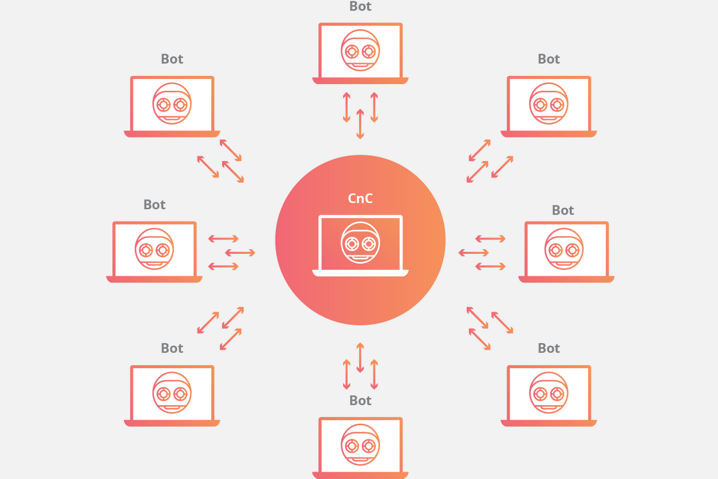
\includegraphics[width=0.50\textwidth]{figuras/botnet}  
  \label{botnet}

\end{figure}

\end{frame}




\begin{frame}{Fases: Recoger información}
  
  \begin{itemize}
  
  \item Se necesita que el dispositivo móvil esté encendido el mayor tiempo posible.   
  
  \item Se necesita una \emph{botnet} para enviar datos de geolocalización
al servidor $\rightarrow$  se crea una instancia de la clase \emph{LocationListener} al comenzar la actividad principal.

  \item Se genera un protocolo para enviar los datos recogidos en una sola cadena. 
  
  \item Es posible transferir los datos recogidos de los \emph{smartphones} a un servidor de dos maneras diferentes
  $\rightarrow$  HTTP o SMS.

  \end{itemize}
\end{frame}

\begin{frame}{Fases: Almacenamiento y gestión de la información}

\begin{itemize}
  
  \item PHP o MySQL para gestionar la información $\rightarrow$  instalados por defectos en la red de servidores mundial.   

  \item Se concatenan todas las variables a almacenar en una única cadena (localización, fecha\ldots). 
  
  \item Primera idea para almacenar los datos: crear para cada \emph{botnet} una nueva tabla con el IMEI (\emph{International Mobile Equipment Identity}) como nombre $\rightarrow$  problema cuando intentamos crear una nueva tabla con un número como nombre (no permitido en MySQL).
  
  \item Solución: traducimos los números de IMEI en caracteres (0 = a, 1 = b, \ldots).  El IMEI es único $\rightarrow$   $n$ tablas con $n$ nombres diferentes.

  \end{itemize}
  
\end{frame}



\begin{frame}{Fases: Mostrar la información}

\begin{itemize}

\item Incluir el encabezado de una web HTML con algunas líneas para inicializar la API de Google Maps.

\item Se inicializa una matriz para tener diferentes colores para nuestros marcadores en el mapa.

\item Consulta SELECT a los IMEIs. Usamos \emph{fecth()} de PHP para acceder a cada línea de la tabla y almacenamos los nombres de tablas en un \emph{array} para poder hacer consultas en todas las tablas de \emph{botnets}.


	\begin{figure}[htbp] 
	\begin{flushright} 
   \includegraphics[width=0.45\textwidth]{figuras/maps}  
  \label{maps}
  \end{flushright}
\end{figure}


\end{itemize}
  
\end{frame}

\begin{frame}{Fases: Información de verificación}

\begin{itemize}
\item Determinar el comportamiento de los dispositivos infectados $\rightarrow$ se debe determinar la velocidad de movimiento de las víctimas.

\item Problema: recopilar suficientes datos para determinar el comportamiento de la víctima.

\item Antes de analizar cualquier comportamiento se debe comprobar los datos $\rightarrow$ se crea una nueva tabla con un nombre que es la concatenación de los nombres de las n tablas separados por "\_". 

\item La fecha será un atributo único en la tabla.


\end{itemize}
  
\end{frame}


\begin{frame}{Fases: Información de verificación}

\begin{itemize}
\item Se puede separar los datos de todas las \emph{botnets} por cualquier periodo de tiempo.

\item Se puede mostrar el mapa datos de las \emph{botnets} respecto a una fecha determinada.

\item Se puede seleccionar y mostrar datos de múltiples objetivos con criterios muy específicos (e.g. la fecha).
\end{itemize}

  	\begin{figure}[htbp] 

   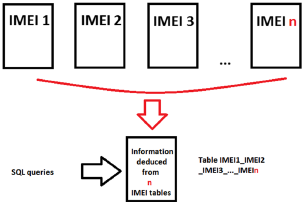
\includegraphics[width=0.45\textwidth]{figuras/IMEIsConcatenados}  
  \label{IMEIsConcatenados}

\end{figure}

\end{frame}

\begin{frame}{Fases: Determinar puntos de encuentro entre dispositivos}

Para predecir la posición de los dispositivos infectados, se utiliza el algoritmo \emph{K-means}. Las características de este algoritmo son:

\begin{itemize}
\item Partición de un conjunto de $N$ observaciones en $K$ grupos.
\item La observación pertenece al grupo con la media más próxima.
\item Computacionalmente difícil de resolver (\emph{NP-hard}).
\end{itemize}
  
\end{frame}

\begin{frame}{Fases: Determinar puntos de encuentro entre dispositivos}

Las fases para determinar la posición son:

\begin{enumerate}
\item Inicialización del algoritmo para obtener datos.
\item \emph{Clustering} con la función \emph{K-means} recursivamente.
\item Inicialización del algoritmo \emph{K-means}.
\item Ejecución del algoritmo \emph{K-means}.
\item Determinación de la posición.
\end{enumerate}

\end{frame}

\section{Conclusiones}

\begin{frame}{Conclusiones}

\begin{itemize}

\item \emph{Botmaster} controla la \emph{botnet}.
\item \emph{Spyware}, \emph{spam}, \emph{DDoS}, robo de información\ldots
\item Aplicación legítima $\rightarrow$ ingeniería inversa $\rightarrow$ aplicación maliciosa.
\item Ejecución en segundo plano (bajo gasto energético y bajo consumo de datos).
\item Predicción de posicionamiento.

\end{itemize}

\end{frame}



\maketitle

\end{document}
